\subsection{Optimisation de \texttt{MetaModel\_impl}}
\label{sec:opti-metamodel}

Les trois optimisations présentées dans cette section ciblent toutes la
classe \texttt{MetaModel\_impl} du bundle \texttt{metadone\_bundle\_metabusiness}.
Elles forment une séquence logique~: la première répare le mécanisme de
cache existant mais inopérant, la deuxième élimine une redondance
algorithmique indépendante du cache, et la troisième rend le cache
efficace pendant le bootstrapping en remplaçant sa stratégie d'invalidation
par une mise à jour incrémentale.

% -------------------------------------------------------------------
\subsubsection{Optimisation~1 : activation du cache et correction de
la clé}
% -------------------------------------------------------------------

L'analyse a révélé que le mécanisme de cache de \texttt{MetaModel\_impl}
était doublement inopérant~: désactivé par construction, et erroné dans
sa gestion des clés. Ces deux défauts ont été corrigés conjointement.

%\paragraph{Activation du cache.}
La classe utilitaire \texttt{CacheCallFunction<Arg,~Ret>} du bundle
\texttt{metadone\_common} associe
à chaque argument une valeur de retour dans une \texttt{HashMap} interne.
Elle accepte un paramètre booléen à la construction qui active ou désactive
ce mécanisme~: lorsqu'il vaut \texttt{false}, chaque appel à
\texttt{isCachedNotNull} retourne systématiquement \texttt{null}, rendant
le cache inopérant sans aucune indication visible à l'appelant. Dans
\texttt{MetaModel\_impl}, ce paramètre était initialisé à \texttt{false},
désactivant globalement le cache de \texttt{getMetaObjectsInDefinition}.
Le premier correctif consiste à passer ce paramètre à \texttt{true}
(figure~\ref{fig:opti-1-cache}).

\begin{figure}[h]
\centering
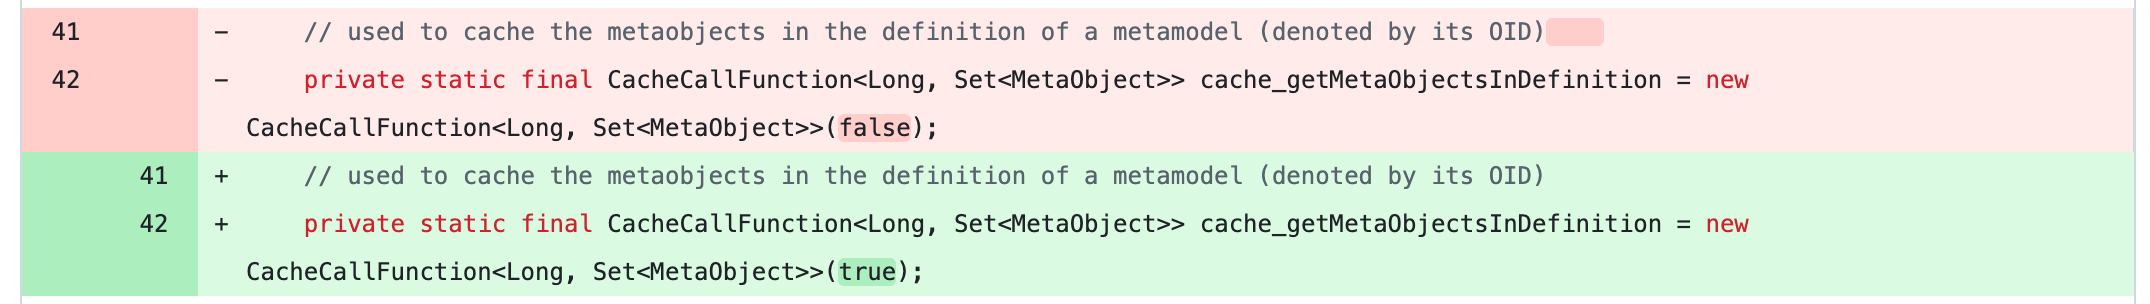
\includegraphics[width=0.9\textwidth]{img/scenario1/opti-1-cache.png}
\caption{Activation du cache \texttt{cache\_getMetaObjectsInDefinition}
dans \texttt{MetaModel\_impl} --- bundle
\texttt{metadone\_bundle\_metabusiness}.}
\label{fig:opti-1-cache}
\end{figure}

%\paragraph{Correction de la clé d'accès.}
Le second défaut porte sur la clé utilisée lors de la consultation du
cache dans \texttt{\_hasInItsDefinition}. \texttt{CacheCallFunction} indexe
ses entrées par l'OID du \texttt{DataObject} sous-jacent : dans ce contexte, la clé naturelle est
l'OID du \texttt{MetaModel} courant (\texttt{this}), puisque le cache
enregistre \textit{l'ensemble des membres de ce MetaModel}.

Or, le code original passait l'OID du \texttt{MetaObject} \textit{recherché}
(\texttt{mo}) à la place. Cette inversion produisait un \textit{cache miss}
systématique~: même si le cache avait contenu l'entrée attendue, elle
n'aurait jamais été trouvée. Le second correctif substitue donc l'OID de
\texttt{this} à celui de \texttt{mo} (figure~\ref{fig:opti-1-cle}).

\begin{figure}[h]
\centering
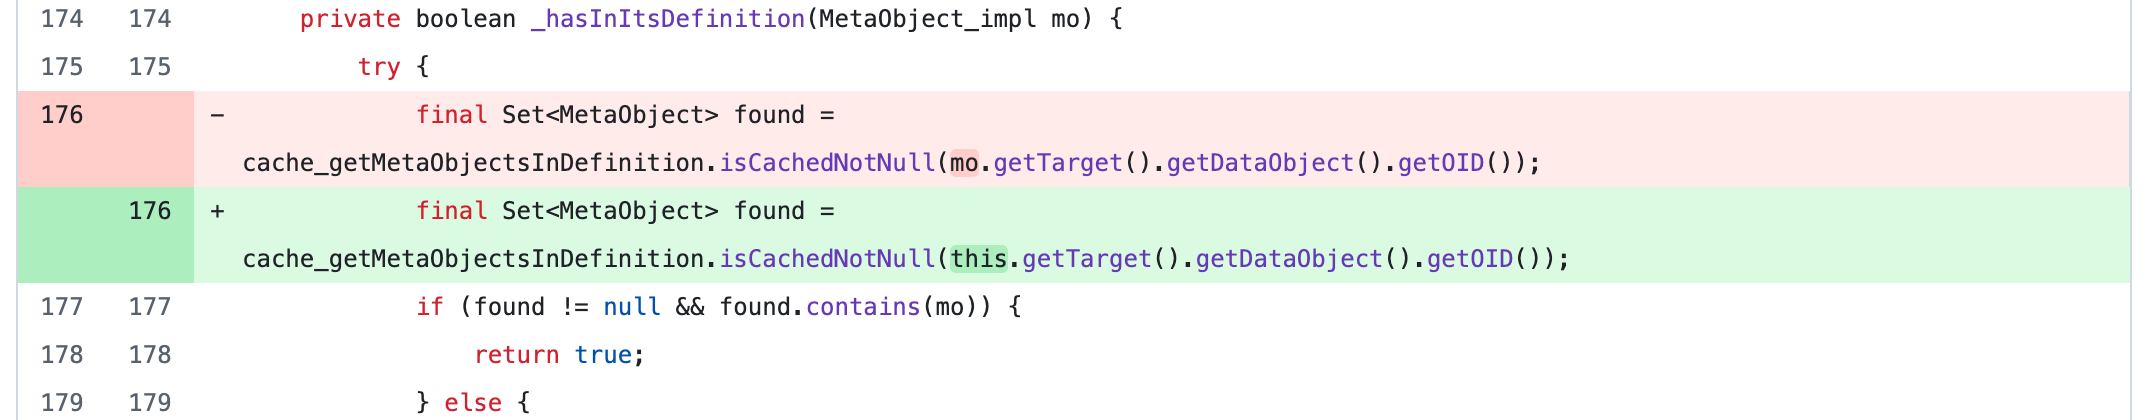
\includegraphics[width=0.9\textwidth]{img/scenario1/opti-1-cle.png}
\caption{Correction de la clé d'accès au cache dans
\texttt{\_hasInItsDefinition} --- l'OID de \texttt{this} (le
\texttt{MetaModel}) se substitue à l'OID de \texttt{mo} (le
\texttt{MetaObject} recherché).}
\label{fig:opti-1-cle}
\end{figure}

%\paragraph{Portée de cette optimisation.}
Ces corrections sont un prérequis logique, mais leur bénéfice est nul
\textit{pendant le bootstrapping}. Lors de la création de la base de
données, les entrées du cache sont systématiquement absentes au moment
où \texttt{\_hasInItsDefinition} est appelé~: chaque appel à
\texttt{\_addInDefinition} invalide le cache avant que le prochain appel
à \texttt{getMetaObjectsInDefinition} ne puisse le peupler. Elles sont
en revanche indispensables pour le bon fonctionnement des optimisations
suivantes, et bénéficient à toutes les requêtes effectuées \textit{après}
le bootstrapping.

% -------------------------------------------------------------------
\subsubsection{Optimisation~2 : suppression de la redondance dans
\texttt{getMOByName}}
% -------------------------------------------------------------------

%\paragraph{Contexte et problème.}
La méthode \texttt{getMOByName} est appelée lors du bootstrapping pour
vérifier l'unicité du nom de chaque nouvel objet ajouté au métamodèle.
Elle itère sur l'ensemble des \texttt{MetaObject} retournés par
\texttt{getMetaObjectsInDefinition()} et, pour chaque élément, invoque
\texttt{mo.getName(this)} afin d'en récupérer le nom.

Conformément au patron \textit{Design by Contract} décrit à la
section~\ref{sec:dbc}, \texttt{getName} est la méthode publique de
l'interface. Avant de déléguer à \texttt{\_getName}, elle effectue deux
vérifications défensives~: un contrôle de nullité, puis une vérification
d'appartenance via \texttt{metamodel.hasInItsDefinition(this)}
(Listing~\ref{ls-getname}, ligne~354--355). Cette précondition appelle à
son tour \texttt{\_hasInItsDefinition}, qui --- sans cache actif ---
déclenche un scan linéaire $O(n)$ via
\texttt{findMetaObjectsInDefinition\_oneshot}.

\begin{lstlisting}[firstnumber=352,
  caption={\texttt{getName} --- méthode publique de \texttt{MetaObject\_impl},
  bundle \texttt{metadone\_bundle\_metabusiness}. La précondition
  ligne~354--355 déclenche un scan $O(n)$ à chaque appel.},
  label={ls-getname}]
@Override
public String getName(MetaModel metamodel) throws BadPreCondition {
    NullArgument.check(metamodel);
    if (!metamodel.hasInItsDefinition(this)) {
        throw new BadPreCondition("Attempt to get the name of a "
            + "metaobject in the context of a metamodel that "
            + "doesn't contain it.");
    }
    try {
        final String result = _getName(metamodel);
        if (result != null) {
            return result;
        }
        throw new Metal2Exception(...);
    } catch (final BadPreCondition e) {
        throw new Metal2Exception(e);
    }
}
\end{lstlisting}

\texttt{\_getName} est la méthode interne qui effectue la recherche
réelle~: elle parcourt les \texttt{ConcreteProperty<String>} associées
au \texttt{MetaObject} et cherche celle définie dans le
\texttt{ConcreteModel} correspondant au \texttt{MetaModel}
(Listing~\ref{ls--getname}, lignes~378--379), puis remonte
récursivement dans les supertypes directs si aucune propriété ne
correspond (ligne~383). Elle ne comporte aucune vérification
d'appartenance.

\begin{lstlisting}[firstnumber=370,
  caption={\texttt{\_getName} --- méthode interne de
  \texttt{MetaObject\_impl}. Pas de vérification d'appartenance~:
  l'invariant est supposé garanti par l'appelant.},
  label={ls--getname}]
private String _getName(MetaModel metamodel) {
    try {
        assert metamodel != null;
        final ConcreteObject thisConcrete = this.narrow2ConcreteObject();
        final ConcreteModel concreteModel =
            metamodel.narrow2ConcreteModel();
        final MetaPropertyExt<String> metaObjectName =
            workspace.getMetaObjectName();
        for (final ConcreteProperty<String> cp :
                thisConcrete.getProperties(metaObjectName)) {
            if (concreteModel.isInDefinition(cp)) {
                return cp.getValue();
            }
        }
        for (final MetaObject mmO : metamodel.getDirectSupertypes()) {
            final MetaModel mm;
            try {
                mm = mmO.narrow(MetaModel.class);
            } catch (final BadPreCondition e) {
                continue;
            }
            final String name = _getName(mm);
            if (name != null) {
                return name;
            }
        }
        return null;
    } catch (final BadPreCondition e) {
        throw new Metal2Exception(e);
    }
}
\end{lstlisting}

%\paragraph{Analyse de la complexité.}
Invoquer \texttt{getName} depuis une boucle sur
\texttt{getMetaObjectsInDefinition()} est structurellement redondant.
Puisque chaque élément \texttt{mo} provient par définition des membres
du \texttt{MetaModel}, la précondition \texttt{hasInItsDefinition(this)}
est toujours vraie et son évaluation est superflue. Sans cache actif, cette
vérification déclenche à chaque itération un parcours de la hiérarchie de
supertypes du \texttt{MetaModel}, chacun de ces supertypes déclenchant à
son tour un scan linéaire dans \texttt{findMetaObjectsInDefinition\_oneshot}.
Le coût cumulé de la boucle est donc~:
\[
\underbrace{O(n)}_{\text{itérations de \texttt{getMOByName}}}
\;\times\;
\underbrace{O(s)}_{\text{supertypes dans \texttt{\_hasInItsDefinition}}}
\;\times\;
\underbrace{O(n)}_{\text{scan dans \texttt{\_oneshot}}}
\;=\; O(n^2 \cdot s)
\]
où $s$ désigne la profondeur de la hiérarchie de supertypes du
\texttt{MetaModel}. La réflexivité de MetaL$_2$ (section~\ref{sec:metal2})
autorise cette profondeur à croître linéairement avec le nombre de
méta-modèles définis~: dans le pire cas, $s = O(n)$, ce qui ramène la
complexité effective à $O(n^3)$ pour la dimension d'appartenance.

%\paragraph{Solution.}
La solution consiste à court-circuiter la méthode publique \texttt{getName}
et à appeler directement \texttt{\_getName}, dont l'invariant d'appartenance
est ici garanti structurellement~: la source des \texttt{MetaObject} est
interne à \texttt{getMOByName}, qui les obtient lui-même via
\texttt{getMetaObjectsInDefinition()}. Pour rendre cet accès possible sans
briser l'encapsulation du bundle, la visibilité de \texttt{\_getName} a été
élargie de \texttt{private} à \textit{package-private}~: les deux classes
\texttt{MetaModel\_impl} et \texttt{MetaObject\_impl} appartenant au même
package, l'accès reste confiné à la couche d'implémentation et invisible
depuis les interfaces publiques de MetaL$_2$.

L'appel est précédé d'un \texttt{narrow(MetaObject\_impl.class)} pour
descendre du type d'interface \texttt{MetaObject} vers l'implémentation
concrète, conformément au patron \textit{Proxy} décrit à la
section~\ref{sec:proxy} (figure~\ref{fig:opti-2}).

\begin{figure}[h]
\centering
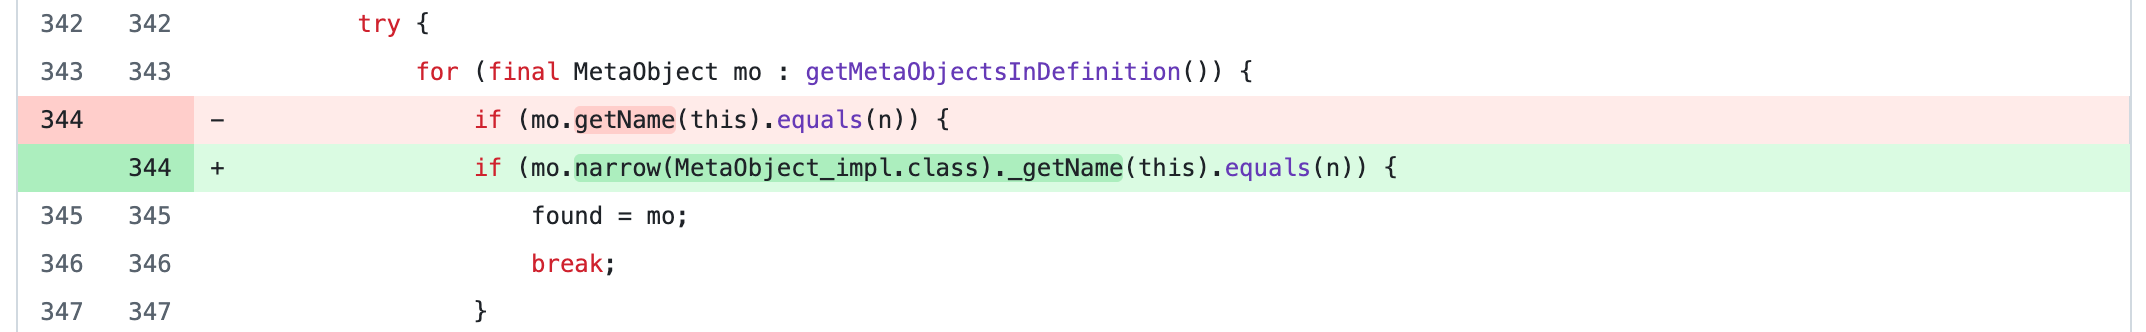
\includegraphics[width=0.9\textwidth]{img/scenario1/opti-2.png}
\caption{Appel direct à \texttt{\_getName} dans \texttt{getMOByName}
--- bundle \texttt{metadone\_bundle\_metabusiness}. Le
\texttt{narrow(MetaObject\_impl.class)} descend du type d'interface
vers l'implémentation concrète selon le patron Proxy.}%(section~\ref{sec:proxy})
\label{fig:opti-2}
\end{figure}

Chaque itération de la boucle passe d'un coût $O(n)$ à un coût
quasi-constant, ramenant le coût cumulé du bootstrapping de $O(n^3)$ à
$O(n^2)$. Notons que le bootstrapping reste $O(n^2)$~: il est nécessaire
de vérifier l'unicité du nom de chaque nouvel objet par rapport aux $n$
objets déjà présents, mais la troisième dimension de complexité --- le
scan d'appartenance --- est supprimée.

Comme le montre la figure~\ref{fig:ouverture-2}, cette seule optimisation divise le temps de création du repository par environ quatre (18\,198~ms $\rightarrow$ 4\,560~ms en médiane, CV~$=$~0,7\,\%).

\begin{figure}[h]
\centering
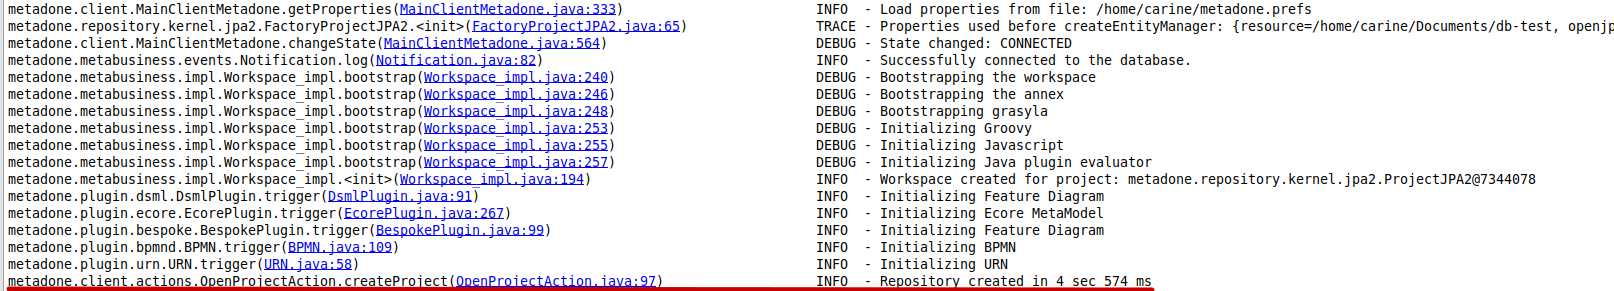
\includegraphics[width=0.9\textwidth]{img/scenario1/ouverture-2.png}
\caption{Temps de création du repository après l'optimisation~2~:
médiane à 4\,560~ms (CV~$=$~0,7\,\%), soit un facteur de réduction de~$\times$\,4,0 par rapport à la baseline de 18\,198~ms.}
\label{fig:ouverture-2}
\end{figure}

% -------------------------------------------------------------------
\subsubsection{Optimisation~3 : mise à jour incrémentale du cache dans
\texttt{\_addInDefinition}}
% -------------------------------------------------------------------

%\paragraph{Problème résiduel.}
Malgré l'activation du cache (optimisation~1), celui-ci reste inefficace
pendant le bootstrapping. La raison est la stratégie d'invalidation
appliquée dans \texttt{\_addInDefinition}~: chaque ajout d'un
\texttt{MetaObject} à la définition d'un \texttt{MetaModel} efface
l'entrée de cache correspondante. Pendant le bootstrapping, où des centaines
d'objets sont ajoutés séquentiellement, cette stratégie condamne le cache
à rester perpétuellement vide~: chaque invalidation supprime l'entrée avant
que le prochain appel à \texttt{getMetaObjectsInDefinition} ne puisse
l'exploiter. Tout appel à \texttt{\_hasInItsDefinition} déclenche donc
toujours un scan $O(n)$ via \texttt{findMetaObjectsInDefinition\_oneshot},
sans jamais bénéficier du cache.

%\paragraph{Solution.}
Le correctif consiste à remplacer la stratégie d'\textbf{invalidation} par
une stratégie de \textbf{mise à jour incrémentale}. La méthode
\texttt{isCached} de \texttt{CacheCallFunction} retourne une paire
\texttt{(Boolean,~Set<MetaObject>)} indiquant si une entrée de cache existe
pour ce \texttt{MetaModel} et, le cas échéant, l'ensemble des membres déjà
mis en cache. Deux cas sont alors distingués (figure~\ref{fig:opti-3})~:

\begin{itemize}
    \item \textbf{Le cache existe}~: le nouvel objet est inséré directement
    dans l'ensemble en mémoire en $O(1)$, maintenant l'invariant du cache
    sans aucun scan supplémentaire.
    \item \textbf{Le cache n'existe pas encore}~: aucune action n'est
    entreprise. Le cache est construit de manière \textit{paresseuse}~:
    c'est le prochain appel à \texttt{getMetaObjectsInDefinition} qui
    effectuera le scan complet et construira l'entrée initiale, en incluant
    tous les objets déjà présents à ce moment.
\end{itemize}

\begin{figure}[h]
\centering
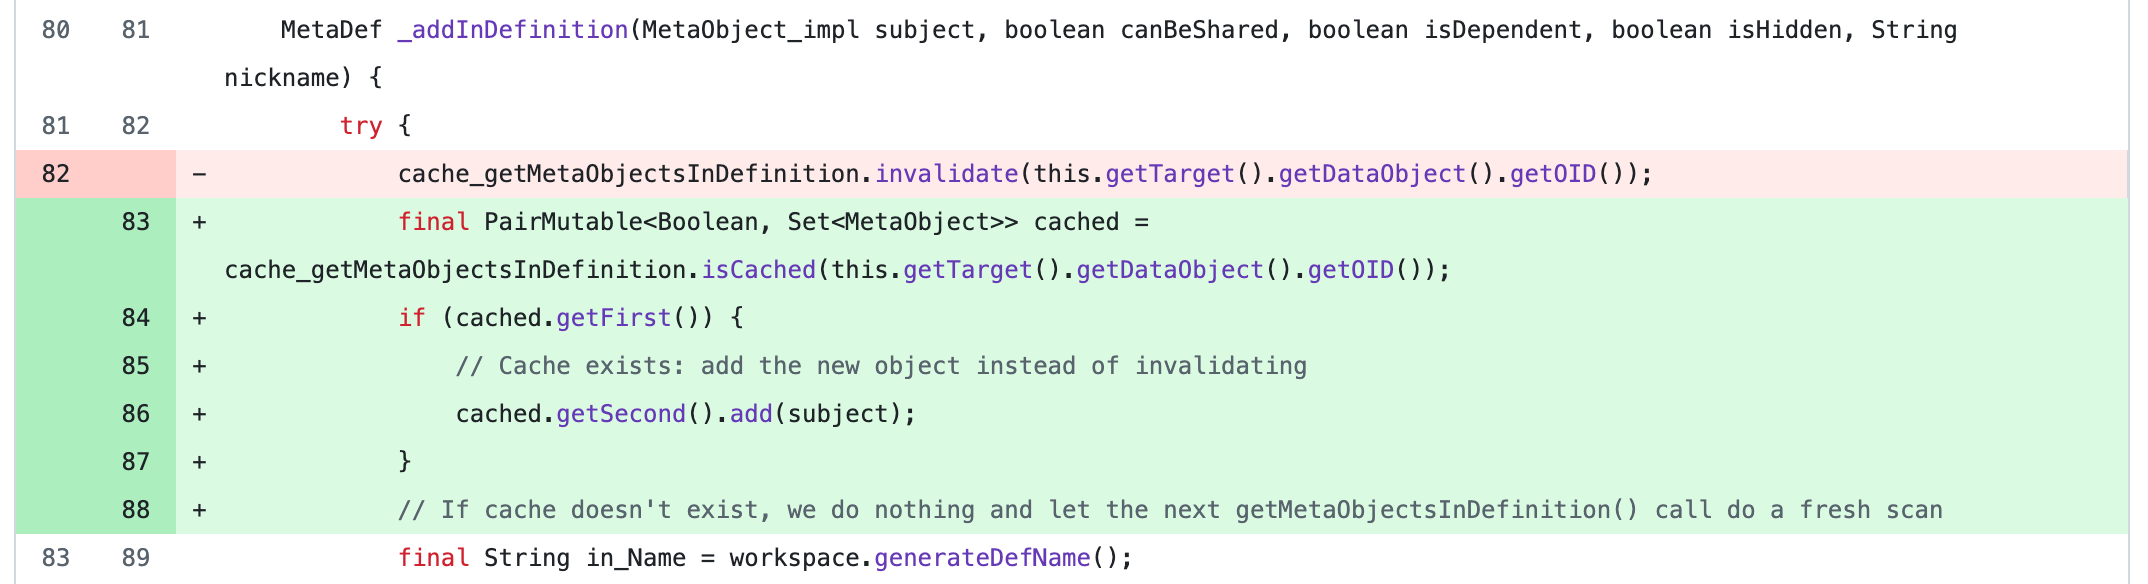
\includegraphics[width=0.9\textwidth]{img/scenario1/opti-3.png}
\caption{Mise à jour incrémentale du cache dans
\texttt{\_addInDefinition} --- bundle
\texttt{metadone\_bundle\_metabusiness}. Deux branches~: insertion
$O(1)$ si le cache existe, initialisation paresseuse sinon.}
\label{fig:opti-3}
\end{figure}

%\paragraph{Correction de la stratégie.}
Cette approche est correcte car l'ensemble mis en cache représente
exactement les membres de la définition du \texttt{MetaModel}~: lors d'un
ajout, on connaît précisément l'élément à insérer, ce qui suffit à maintenir
la cohérence sans reconstruire l'ensemble. La stratégie d'initialisation
paresseuse garantit par ailleurs qu'aucun cache partiellement construit
n'est jamais consulté~: soit le cache est complet (construit par un appel
antérieur à \texttt{getMetaObjectsInDefinition}), soit il est absent et
sera reconstruit à la demande.

%\paragraph{Interaction avec l'optimisation~1.}
Cette optimisation ne peut fonctionner correctement que si le cache est
activé (optimisation~1) et que la clé utilisée est la bonne. Les trois
optimisations forment donc une chaîne dépendante~: l'optimisation~1 est
un prérequis pour que les optimisations~2 et~3 aient un effet, et
l'optimisation~3 est ce qui rend le cache efficace \textit{pendant} le
bootstrapping plutôt que seulement après.

La combinaison des trois optimisations transforme les scans $O(n)$
répétés en de simples insertions et lectures mémoire $O(1)$, réduisant
la complexité algorithmique du bootstrapping de $O(n^3)$ à $O(n^2)$
pour la dimension d'appartenance.

\subsection{Tests de performance}
\label{sec:scenario1-tests1}

Conformément au cycle décrit à la section~\ref{sec:cycle}, les
optimisations implémentées sont évaluées par comparaison avec la
\textit{baseline} établie à la section~\ref{sec:scenario1}
(18~198~ms). Deux dimensions sont mesurées~: le \textbf{volume d'appels}
dans la chaîne critique (via l'instrumentation manuelle par compteurs),
et le \textbf{profil CPU} après optimisation (via JFR et async-profiler).

% -----------------------------------------------
\subsubsection{Réduction du volume d'appels}
% -----------------------------------------------

Le tableau~\ref{tab:appels-opti1} résume l'évolution du nombre d'appels
dans la chaîne critique pour une charge de travail identique (bootstrapping
complet du repository avec le plugin BPMN).

\begin{table}[h]
\centering
\caption{Évolution du volume d'appels dans la chaîne critique ---
bootstrapping complet du repository.}
\label{tab:appels-opti1}
\begin{tabular}{lrrr}
\hline
\textbf{Méthode} & \textbf{Avant} & \textbf{Après} &
\textbf{Réduction} \\
\hline
\texttt{\_hasInItsDefinition} & $\sim$1~400 & $\sim$650 & $\sim$54\% \\
\texttt{findMetaObjectsInDefinition\_oneshot} & $\sim$80~000 & $\sim$750 &
$\sim$99\% \\
\hline
\end{tabular}
\end{table}

La réduction de 54\% des appels à \texttt{\_hasInItsDefinition} est la
conséquence directe de l'\textbf{optimisation~1}~: le cache étant désormais
opérationnel avec la bonne clé, une fraction significative des vérifications
d'appartenance est court-circuitée dès que l'information est disponible en
mémoire, sans traversée du graphe.

L'impact le plus massif est celui de l'\textbf{optimisation~2}~: la chute
de 99\% des appels à \texttt{findMetaObjectsInDefinition\_oneshot} confirme
que la suppression de la précondition dans \texttt{getMOByName} a brisé la
boucle quadratique. Le système ne répercute plus un scan $O(n)$ sur chaque
accès au nom d'un objet~; la troisième dimension de complexité est
éliminée.

L'\textbf{optimisation~3} contribue au reliquat~: grâce à la mise à jour incrémentale, les appels qui atteignent encore \texttt{\_hasInItsDefinition} sont servis en $O(1)$ depuis le cache au lieu de redéclencher un parcours complet de \texttt{getRangeOf}.

% -----------------------------------------------
\subsubsection{Profilage post-optimisation avec JFR}
% -----------------------------------------------

La figure~\ref{fig:jfr-2} montre le Method Profiling JMC après
optimisation. Le compteur d'échantillons pour la chaîne critique est passé
de 163 à 28, et \texttt{getModel} --- qui dominait avec 52,1\% des
échantillons CPU --- n'en représente plus que 7,14\%. Ces chiffres
confirment que le goulot d'étranglement identifié à la
section~\ref{sec:scenario1-profil1} a été résolu~: la méthode n'apparaît
plus en tête du classement de charge.

\begin{figure}[h]
\centering
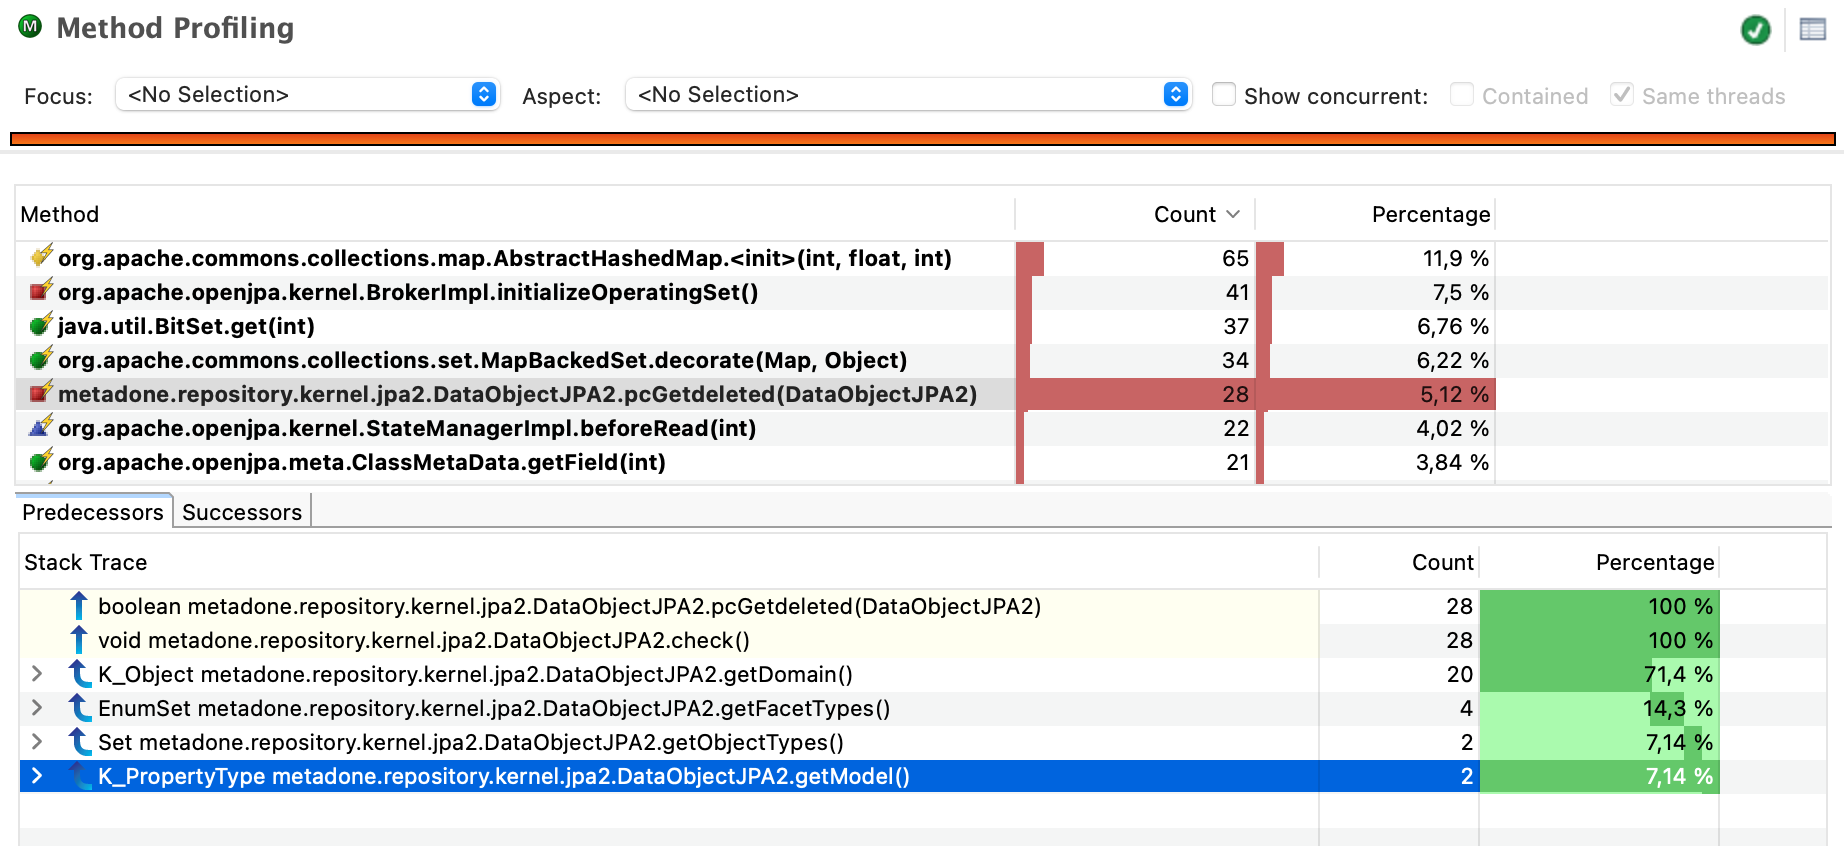
\includegraphics[width=0.9\textwidth]{img/scenario1/jfr-2.png}
\caption{Java Mission Control --- Method Profiling après optimisation.
Le compteur de la chaîne critique passe de 163 à 28 échantillons~;
\texttt{getModel} (bundle \texttt{metadone\_bundle\_repository\_jpa2})
tombe de 52,1\% à 7,14\% de charge CPU.}
\label{fig:jfr-2}
\end{figure}

% -----------------------------------------------
\subsubsection{Profilage post-optimisation avec async-profiler}
% -----------------------------------------------

Les flamegraphs de la figure~\ref{fig:prof2-zoom} isolent les mêmes
méthodes que celles analysées à la section~\ref{sec:scenario1-profil1},
permettant une comparaison directe avant/après.

\texttt{findMetaObjectsInDefinition\_oneshot}
(figure~\ref{fig:prof2-oneshot}) ne domine plus la pile d'appels~: sa
largeur dans le flamegraph est désormais négligeable, indiquant que les
traversées de \texttt{getRangeOf} dans le bundle
\texttt{metadone\_bundle\_repository} ont quasi disparu de la charge CPU
mesurée. Les opérations qui occupent maintenant le profil correspondent
à la construction légitime des objets du métamodèle, non plus à des
vérifications redondantes.

\begin{figure}[htbp]
\begin{subfigure}{\textwidth}
    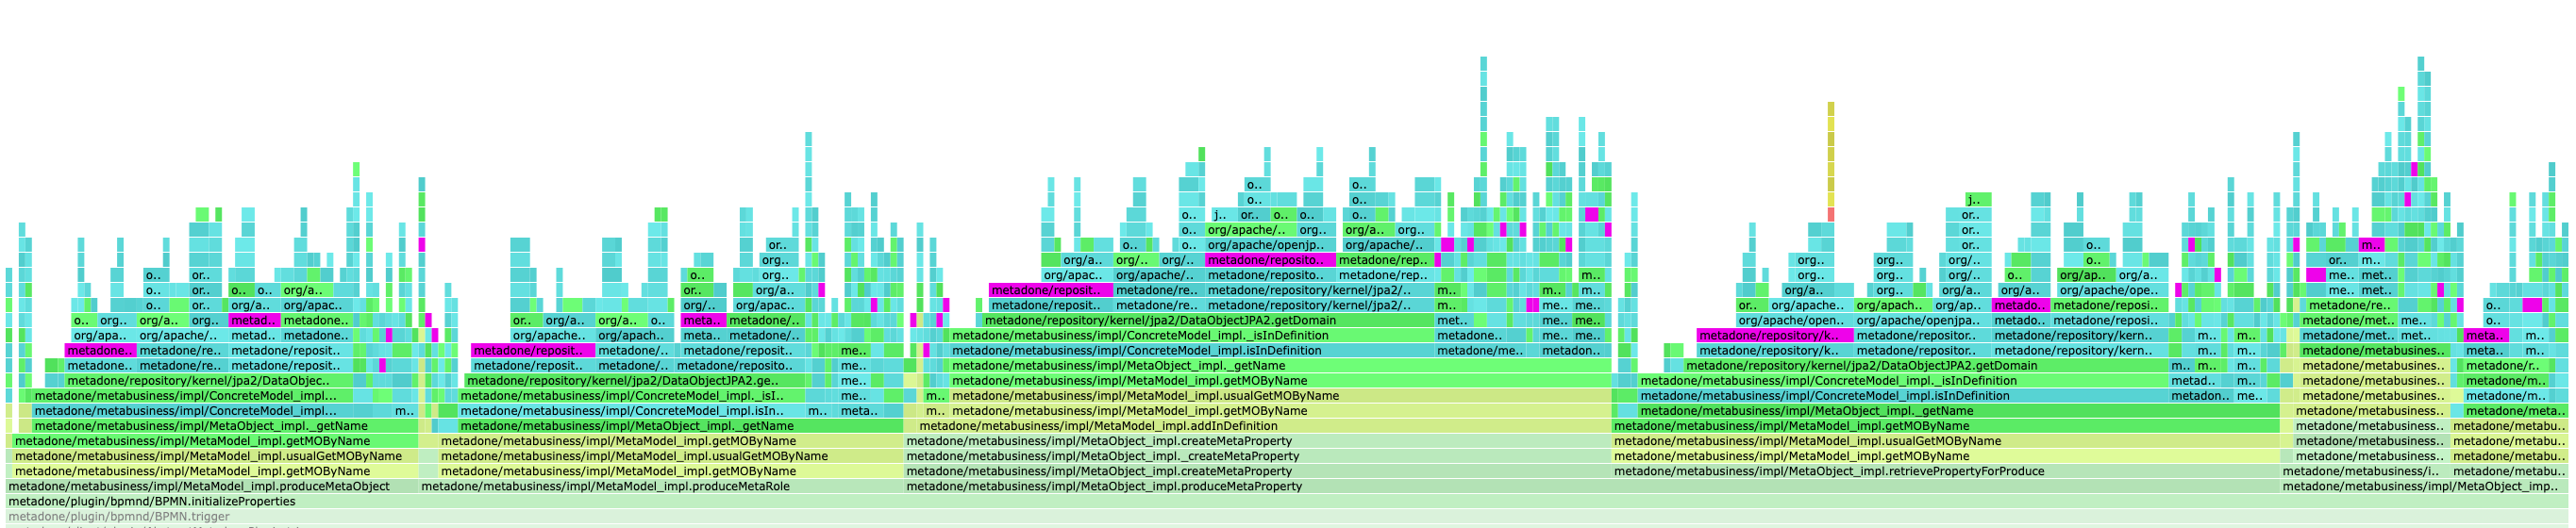
\includegraphics[width=\textwidth]{img/scenario1/prof2/pcGetdeleted.png}
    \caption{\texttt{pcGetdeleted} ---
    bundle \texttt{metadone\_bundle\_repository\_jpa2}}
    \label{fig:prof2-pcGetdeleted}
\end{subfigure}

\medskip
\begin{subfigure}{\textwidth}
    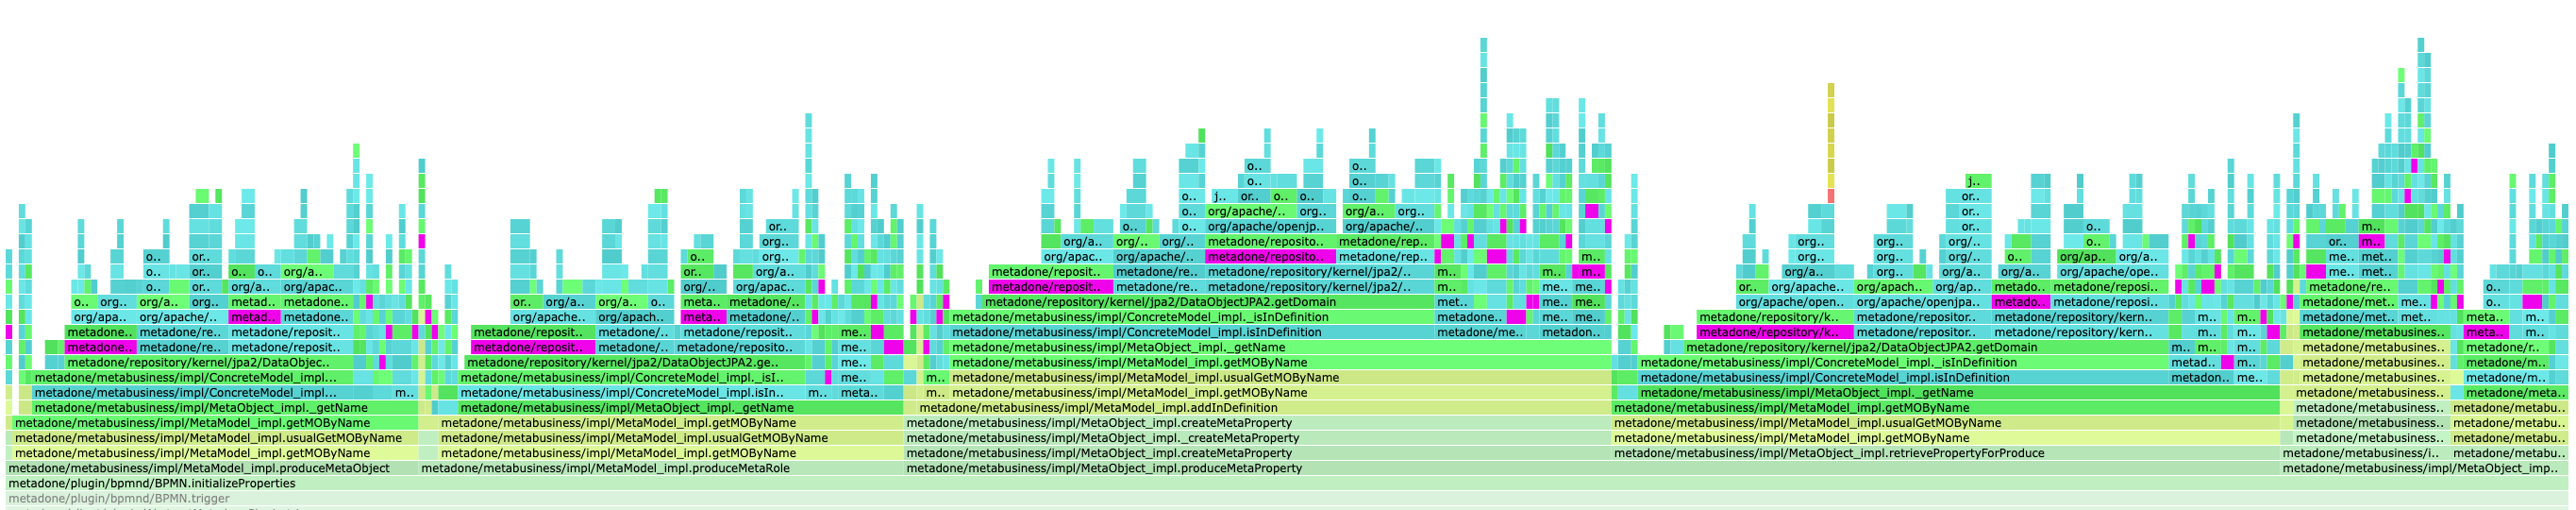
\includegraphics[width=\textwidth]{img/scenario1/prof2/check.png}
    \caption{\texttt{check} ---
    bundle \texttt{metadone\_bundle\_repository\_jpa2}}
    \label{fig:prof2-check}
\end{subfigure}

\medskip
\begin{subfigure}{\textwidth}
    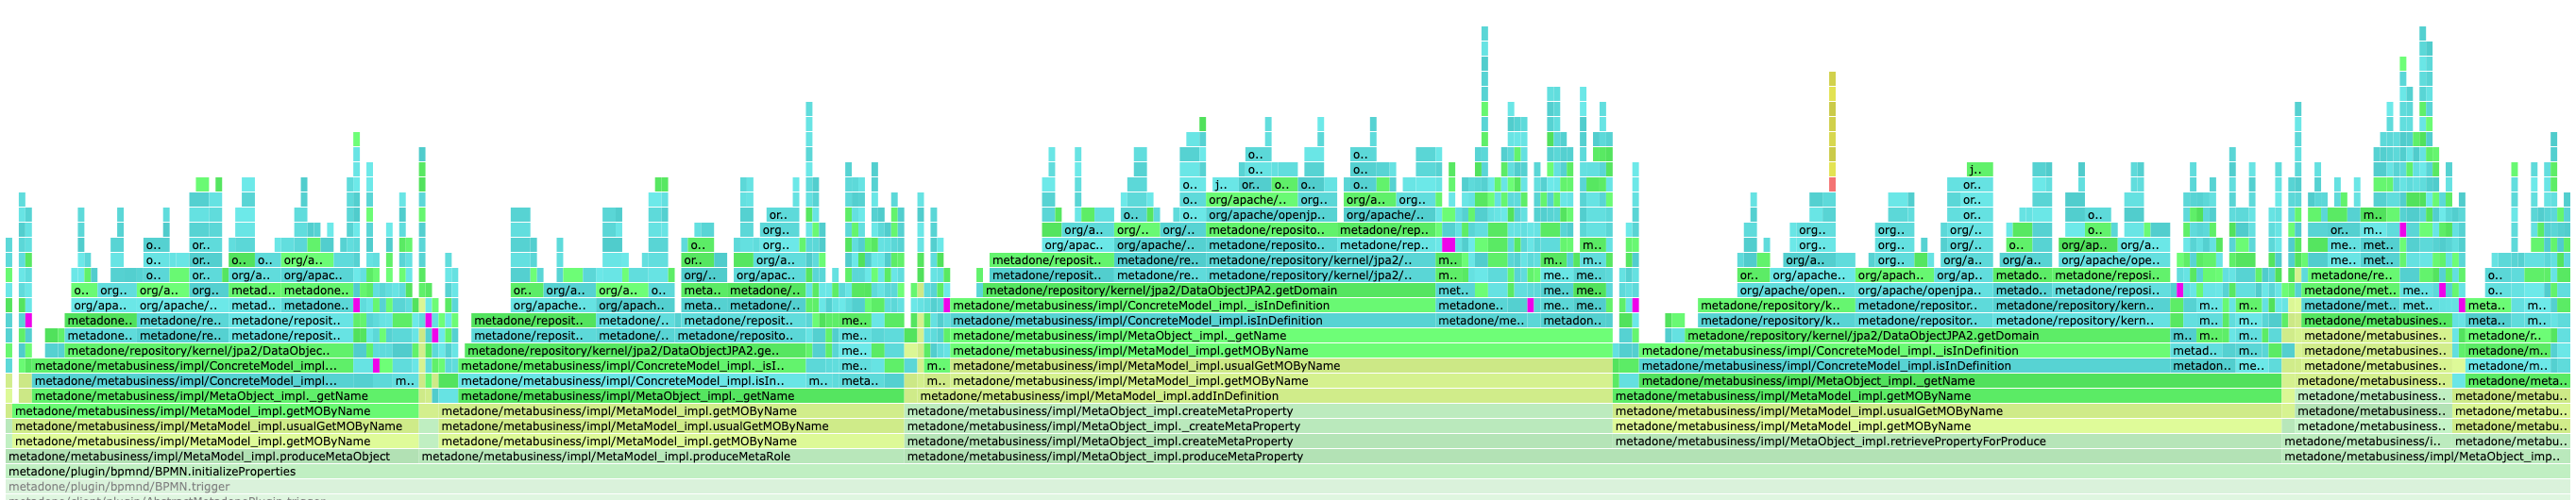
\includegraphics[width=\textwidth]{img/scenario1/prof2/getModel.png}
    \caption{\texttt{getModel} ---
    bundle \texttt{metadone\_bundle\_repository\_jpa2}}
    \label{fig:prof2-getModel}
\end{subfigure}

\medskip
\begin{subfigure}{\textwidth}
    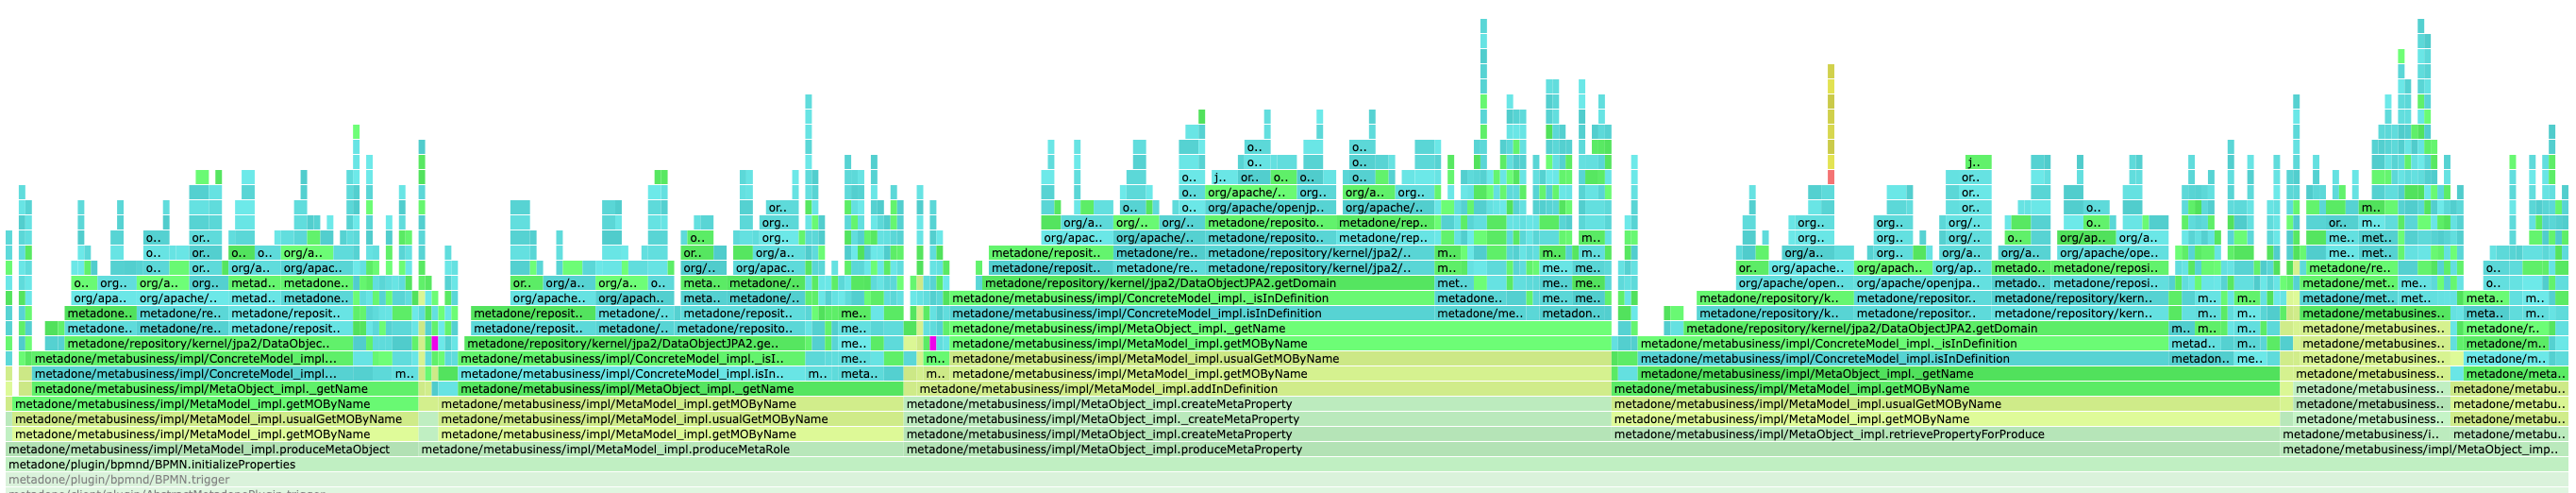
\includegraphics[width=\textwidth]{img/scenario1/prof2/getRangeOf.png}
    \caption{\texttt{getRangeOf} --- interface \texttt{K\_Object},
    bundle \texttt{metadone\_bundle\_repository}
    }
    \label{fig:prof2-getRangeOf}
\end{subfigure}

\medskip
\begin{subfigure}{\textwidth}
    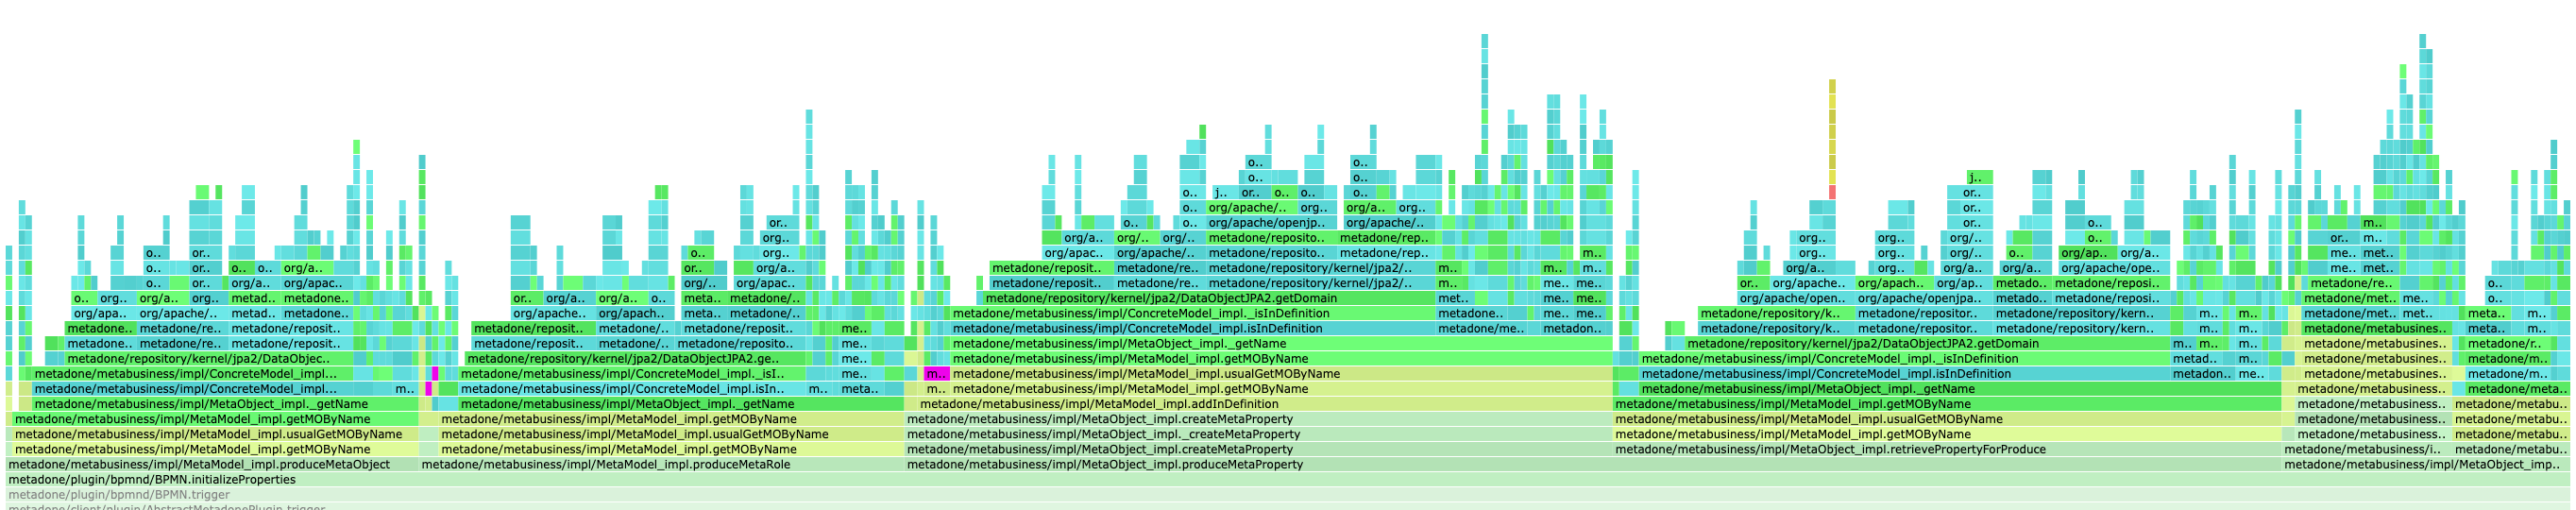
\includegraphics[width=\textwidth]{img/scenario1/prof2/oneshot.png}
    \caption{\texttt{findMetaObjectsInDefinition\_oneshot} ---
    classe \texttt{MetaModel\_impl},
    bundle \texttt{metadone\_bundle\_metabusiness}
    }
    \label{fig:prof2-oneshot}
\end{subfigure}

\caption{Flamegraphs post-optimisation --- même périmètre que la
figure~\ref{fig:prof1-zoom}. L'occupation CPU de
\texttt{findMetaObjectsInDefinition\_oneshot} et de la chaîne
\texttt{getRangeOf} $\to$ \texttt{getModel} $\to$ \texttt{check} $\to$
\texttt{pcGetdeleted} est désormais négligeable.}
\label{fig:prof2-zoom}
\end{figure}

% -----------------------------------------------
\subsubsection{Bilan du premier cycle d'optimisation}
% -----------------------------------------------

Le tableau~\ref{tab:bilan-opti1} synthétise les gains mesurés à l'issue
de ce premier cycle.

\begin{table}[h]
\centering
\caption{Bilan du premier cycle d'optimisation --- scénario
d'initialisation. Les médianes sont calculées sur 10 répétitions avec un
coefficient de variation inférieur à 1\,\% (mesures complètes en
annexe~\ref{ann:mesures-s1-a}).}
\label{tab:bilan-opti1}
\begin{tabular}{lrr}
\hline
\textbf{Indicateur} & \textbf{Baseline} & \textbf{Après opti.~1--3} \\
\hline
Temps de démarrage (médiane) & 18\,198~ms & 4\,516~ms \\
Facteur de réduction & --- & $\times$\,4,0 \\
Appels \texttt{findMetaObjectsInDefinition\_oneshot} & $\sim$80\,000 &
$\sim$750 \\
Charge CPU \texttt{getModel} (JFR) & 52,1\,\% & 7,14\,\% \\
Complexité algorithmique (dimension appartenance) & $O(n^2 \cdot s)$ & $O(n^2)$
\\
\hline
\end{tabular}
\end{table}

Au-delà du gain brut d'un facteur~4,0, ces modifications transforment
la \textbf{courbe de scalabilité} de MetaDONE. La version initiale
présentait une croissance en $O(n^2 \cdot s)$ du temps de bootstrapping
(cubique dans le pire cas où la hiérarchie de supertypes est profonde,
$s = O(n)$)~; la version optimisée ramène cette croissance à $O(n^2)$.
Cette différence est qualitative~: pour un métamodèle deux fois plus
grand, le coût ne croît plus selon la profondeur de la hiérarchie de
supertypes, rendant l'outil viable sur des modèles de grande envergure
là où l'architecture initiale l'aurait rendu impraticable.

Un goulot d'étranglement résiduel demeure néanmoins visible dans les
flamegraphs~: \texttt{pcGetdeleted} et \texttt{getRangeOf} conservent
une présence non négligeable dans la pile CPU, indiquant que les accès
au dépôt JPA restent coûteux indépendamment du cache applicatif. Ce
point constitue la piste d'investigation du prochain cycle d'analyse.